% !TEX encoding = UTF-8 Unicode
\documentclass[
10pt,
aspectratio=169,
]{beamer}
\setbeamercovered{transparent=10}
\usetheme[
%  showheader,
%  red,
  purple,
%  gray,
%  graytitle,
  colorblocks,
%  noframetitlerule,
]{Verona}

\usepackage[T1]{fontenc}
\usepackage[utf8]{inputenc}
\usepackage{lipsum}
%%%%%%%%%%%%%%%%%%%%%%%%%%%%%%%
% Mac上使用如下命令声明隶书字体,windows也有相关方式,大家可自行修改
%\providecommand{\lishu}{\CJKfamily{zhli}}
%%%%%%%%%%%%%%%%%%%%%%%%%%%%%%%
\usepackage{tikz}
\usetikzlibrary{shapes,arrows,positioning,shadows}
\usetikzlibrary{fadings}
%
%\setbeamertemplate{sections/subsections in toc}[ball]
%\usepackage{xeCJK}
%\ProvidesPackage{minted}
\usepackage{minted}
\usepackage{adjustbox} % Shrink stuff
\usepackage{listings}
\usepackage{caption}
\usepackage{subcaption}
\usefonttheme{professionalfonts}
\def\mathfamilydefault{\rmdefault}
\usepackage{amsmath}
\usepackage{multirow}
\usepackage{booktabs}
\usepackage{bm}
\setbeamertemplate{section in toc}{\hspace*{1em}\inserttocsectionnumber.~\inserttocsection\par}
\setbeamertemplate{subsection in toc}{\hspace*{2em}\inserttocsectionnumber.\inserttocsubsectionnumber.~\inserttocsubsection\par}
\setbeamerfont{subsection in toc}{size=\small}
\AtBeginSection[]{%
	\begin{frame}%
		\frametitle{Outline}%
		\textbf{\tableofcontents[currentsection]} %
	\end{frame}%
}

% Commands
\newcommand{\bftt}[1]{\textbf{\texttt{#1}}}
%\newcommand{\cmd}[1]{{\color[HTML]{008000}\bftt{#1}}}
%\newcommand{\comment}[1]{{\color[HTML]{008080}\textit{\textbf{\texttt{#1}}}}}
\newcommand{\cmd}[1]{{\color[HTML]{008000}\bftt{#1}}}
\newcommand{\bs}{\char`\\}
\newcommand{\cmdbs}[1]{\cmd{\bs#1}}
\newcommand{\lcb}{\char '173}
\newcommand{\rcb}{\char '175}
\newcommand{\cmdbegin}[1]{\cmdbs{begin\lcb}\bftt{#1}\cmd{\rcb}}
\newcommand{\cmdend}[1]{\cmdbs{end\lcb}\bftt{#1}\cmd{\rcb}}
\newcommand*\keystroke[1]{%
  \tikz[baseline=(key.base)]
    \node[%
      draw,
      fill=white,
      drop shadow={shadow xshift=0.25ex,shadow yshift=-0.25ex,fill=black,opacity=0.75},
      rectangle,
      rounded corners=2pt,
      inner sep=1pt,
      line width=0.5pt,
      font=\scriptsize\sffamily
    ](key) {#1\strut}
  ;
}
\newcommand{\keystrokebftt}[1]{\keystroke{\bftt{#1}}}
\newcommand{\wlnewdoc}[1]{\wlserver/docs?snip\_uri=\fileuri/#1\&splash=none}
\newcommand{\wllogo}{\textbf{Overleaf}}


% Environments
\newenvironment{exampletwoup}
  {\VerbatimEnvironment
   \begin{VerbatimOut}{example.out}}
  {\end{VerbatimOut}
   \setlength{\parindent}{0pt}
   \fbox{\begin{tabular}{l|l}
   \begin{minipage}{0.55\linewidth}
     \inputminted[fontsize=\small,resetmargins]{latex}{example.out}
   \end{minipage} &
   \begin{minipage}{0.35\linewidth}
     \input{example.out}
   \end{minipage}
   \end{tabular}}}

\newenvironment{exampletwouptiny}
  {\VerbatimEnvironment
   \begin{VerbatimOut}{example.out}}
  {\end{VerbatimOut}
   \setlength{\parindent}{0pt}
   \fbox{\begin{tabular}{l|l}
   \begin{minipage}{0.55\linewidth}
     \inputminted[fontsize=\scriptsize,resetmargins]{latex}{example.out}
   \end{minipage} &
   \begin{minipage}{0.35\linewidth}
     \setlength{\parskip}{6pt plus 1pt minus 1pt}%
     \raggedright\scriptsize\input{example.out}
   \end{minipage}
   \end{tabular}}}



\AtBeginSubsection[]{%
	\begin{frame}%
		\frametitle{Outline}%
		\textbf{\tableofcontents[currentsection, currentsubsection]} %
	\end{frame}%
}

\title{Procesadores de texto}
\subtitle{Introduccio\'on a LaTeX y BitTeX}
\author[L.M.]{Luis Alejandro Morales, Ph.D.}
\mail{lmoralesm@unal.edu.co}
\institute[UNAL]{Facultad de Ingenier\'ia, Departamento de Ingnenier\'ia Civil y Agr\'icola\\
Universidad Nacional de Colombia, Bogot\'a}
\date{\today}
\titlegraphic[width=3cm]{logo_01u}{}

%%%%%%%%%%%%%%%%%%%%%%%%%%%%%%%%
% ----------- 标题页 ------------
%%%%%%%%%%%%%%%%%%%%%%%%%%%%%%%%
% New commands
\newcommand{\gi}{\texttt{Git}}
\newcommand{\gih}{\texttt{GitHub}}
\newcommand{\co}[1]{\alert{\textbf{\large \texttt{#1}}}}
\begin{document}



\maketitle

%%% define code
\defverbatim[colored]\lstI{
	\begin{lstlisting}[language=C++,basicstyle=\ttfamily,keywordstyle=\color{red}]
	int main() {
	// Define variables at the beginning
	// of the block, as in C:
	CStash intStash, stringStash;
	int i;
	char* cp;
	ifstream in;
	string line;
	[...]
	\end{lstlisting}
}
%%%%%%%%%%%%%%%%%%%%%%%%%%%%%%%%
% ----------- FRAME ------------
%%%%%%%%%%%%%%%%%%%%%%%%%%%%%%%%

%---
\section{Generalidades}

\begin{frame}[c]{Generalidades}
\begin{itemize}
\item \LaTeX un sistema tipografico.
\item Dise\~nado para scientificos, con especial uso en \alert{matematicas}.
\item Excelente para excribir texto pero ademas para escribir ecuaciones con los mas altos estandares tipograficos para matematicas.
\item Created by \alert{Donald Knuth}
\item \LaTeX fue publicado en \TeX book.
\end{itemize}
\end{frame}


\begin{frame}[c]{¿Como funciona \LaTeX?}
\begin{itemize}
\item \LaTeX llama archivos de estilo, librerias de fuentes, otros paquetes, etc., para crear el estilo deseado.
\item Es de gran alcance y puede extenderse con nuevas librerias.
\item \LaTeX es un \alert{lenguage de programaci\'on} dise\~nado para organizar documentos as preprints, articulos, libros, presentaciones, cartas, etc.
\item Los comandos en \LaTeX son introducidos con  $\backslash$. 
\item \LaTeX se ha constituido en un estandard para producir documentos cientificos.
\end{itemize}
\end{frame}

\begin{frame}[c]{¿Que necesito?}
\begin{itemize}
\item Un \alert{editor} de texto plano. Funciona como un \alert{frond end} E.j. \texttt{Vi/Vim}, \texttt{Emacs}, \texttt{NodePad}, etc. Otros editores disenados para \LaTeX, e.j. \texttt{TeXmaker}, \texttt{TeXStudio}.
\item El sotfware de \LaTeX (\url{https://www.latex-project.org/get/}):
\begin{itemize}
\item Para Linux: \alert{TeX Live}
\item Para Mac OS: \alert{MacTeX}
\item Para Windows: \alert{MiKTeX o TeX Live}
\end{itemize}
\item Tambien es posible usar \alert{Overleaf} (\url{http://www.overleaf.com}) para crear documentos en \LaTeX online.
\end{itemize}

\end{frame}

\begin{frame}[fragile]{¿Cómo trabaja?}
  \begin{itemize}
  \item Escribe tu documento en  \texttt{texto plano} con \cmd{comandos} que describen su estructura y significado.
  \item El programa \texttt{latex} procesa su texto y  comandos para
    producir un documento de alta calidad tipográfica.
  \end{itemize}
  \vskip 2ex
  \begin{center}
    \begin{minted}[frame=single]{latex}
La lluvia en Espa\~na cae \emph{principalmente} 
en la llanura.
    \end{minted}
    \vskip 2ex
    \tikz\node[single arrow,fill=gray,font=\ttfamily\bfseries,%
    rotate=270,xshift=-1em]{latex};
    \vskip 2ex
    \fbox{La lluvia en España cae \emph{principalmente} sobre la llanura.}
  \end{center}
\end{frame}

\begin{frame}[fragile]{Más ejemplos de comandos y sus salidas\ldots}
  \begin{exampletwoup}
\begin{itemize}
\item T\'e
\item Leche
\item Galletas
\end{itemize}
  \end{exampletwoup}
  \vskip 2ex
  \begin{exampletwoup}
\begin{figure}
  
\includegraphics{logo_pe}
\end{figure}
  \end{exampletwoup}
  \vskip 2ex
  \begin{exampletwoup}
\begin{equation}
  \alpha + \beta + 1
\end{equation}
  \end{exampletwoup}
  
%  \tiny{Imagen de \url{http://www.andy-roberts.net/writing/latex/importing_images}}
\end{frame}

\begin{frame}[fragile]{Cambio de concepto en la redacción}
  
  \begin{itemize}
  \item Utilizar comandos para describir ``Qué es'', y no ``Cómo se ve''.
  \item Concentrarse en su contenido.
  \item Deje a \LaTeX{} hacer su trabajo.
  \end{itemize}
\end{frame}

%---
\section{Conceptos Básicos}
\begin{frame}[fragile]{Estructura b\'asica del documento}
  \begin{itemize}
  \item Un documento \LaTeX{} simple:
    \inputminted[frame=single]{latex}{basics.tex}
  \item Los comandos comienzan con una \emph{barra invertida} \keystrokebftt{\bs}.
  \item Todo documento comienza con un comando \cmdbs{documentclass}.
  \item El \emph{argumento} en llaves \keystrokebftt{\{}
    \keystrokebftt{\}} le dice a \LaTeX{} que tipo de documento estamos
    creando: en este ejemplo, \bftt{article}.
  \item Un signo de porcentaje \keystrokebftt{\%} comienza un
    \emph{comentario} --- \LaTeX{} ignorará el resto de la línea.
  \end{itemize}
\end{frame}

\begin{frame}[fragile]{Estructura b\'asica del documento}
  \begin{itemize}
\item \LaTeX distinge el \alert{modo texto} del \alert{modo matematico}.
\item \alert{modo texto} es el modo natural. El compilador establece el tipo de fuente, escoge donde romper lineas y paginas, etc.
\item El compilador toma cualquier numero de espacios entre palabras en el editor como si fuera uno.
 \end{itemize}
\end{frame}

\begin{frame}[fragile]{El \cmdbs{documentclass}}
\begin{itemize}
\item Las opciones en \cmdbs{documentclass} le dicen al compilador acerca del taman\~no de fuente, taman\~no de papel, etc.
\item La clase le indica al compilador que tipo de documento se quiere producir. Clase pueden ser: \alert{book}, \alert{article}, \alert{report}, \alert{beamer} (presentaci\'on)
\end{itemize}
\begin{center}
\large
\cmdbs{documentclass[a4paper,11pt]\{article\}}
\end{center}
\end{frame}

\begin{frame}[fragile]{El preambulo}
\begin{itemize}
\item El preambulo son las lineas siguientes a \cmdbs{documentclass} que proporcionan informacion acerca de preferencias del documento, e.j. paquetes, comandos.
    \inputminted[frame=single]{latex}{basics10.tex}
\end{itemize}
\end{frame}

\begin{frame}[fragile]{Escritura del texto}
  \small
  \begin{itemize}
  \item Escriba su texto entre\cmdbegin{document} y \cmdend{document}.
  \item En su mayoría, puede escribir texto normalmente.
    \begin{exampletwouptiny}
Las palabras se separan por uno 
o m\'as espacios.

Los p\'arrafos se separan por 
uno o m\'as lineas en blanco.
    \end{exampletwouptiny}
  \item Los espacios de más en el archivo fuentes son eliminados en la salida. 
    \begin{exampletwouptiny}
La   lluvia    en Espa\~na
cae principalmente   sobre 
la llanura.
    \end{exampletwouptiny}
  \end{itemize}
\end{frame}


\begin{frame}[fragile]{Escritura de texto: Aclaraciones}
  \small
  \begin{itemize}
  \item Las comillas son un poco complicadas: use el acento invertido
    \keystroke{\`{}} sobre el lado izquierdo y el apóstrofe
    \keystroke{\'{}} sobre el lado derecho.
    \begin{exampletwouptiny}
 Comillas simple: `texto'.

 Comillas dobles: ``texto''.
    \end{exampletwouptiny}
    
  \item Algunos caracteres comunes tienen significados especiales en \LaTeX:\\[1ex]
    \begin{tabular}{cl}
      \keystrokebftt{\%} & Signo de porcentaje \\
      \keystrokebftt{\#} & Signo numeral \\
      \keystrokebftt{\&} & Ampersand                 \\
      \keystrokebftt{\$} & Signo pesos               \\
    \end{tabular}
  \item Si son usados, tendremos errores en la compilación. Si quieres
    que alguno de estos caracteres aparezcan en la salida, se tiene que
    preceder con una barra invertida al caracter.
    \begin{exampletwoup}
\$\%\&\#!
    \end{exampletwoup}
  \end{itemize}
\end{frame}

\begin{frame}[fragile]{Errores de manejo}
  \begin{itemize}
  \item \LaTeX{} puede confundirse cuando está intentando compilar su
    documento. Si esto sucede, se detendrá la compilación por un
    error, y en este caso deberá corregir antes de producir cualquier
    archivo de salida. 
  \item Por ejemplo, si escribe mal \cmdbs{emph} como \cmdbs{meph},
    \LaTeX{} se detendrá con un mensaje de error ``undefined control
    sequence'', ya que ``meph'' no es un comando reconocido.
  \end{itemize}
  \begin{block}{Indicaciones sobre Errores}
    \begin{enumerate}
    \item No se asuste! Los errores suceden.
    \item Corregirlos a medida que se vayan presentando --- si lo que
      acabas de escribir causa un error, puedes comenzar a depurar por ahí.
    \item Si hay múltiples errores, comienza por el primero de ellos
      --- La causa puede incluso estar por arriba de este.
    \end{enumerate}
  \end{block}
\end{frame}

\begin{frame}[fragile]{Ejercicio de Tipografía 1}
  \begin{block}{Escriba esto en \LaTeX:
      \footnote{\url{http://en.wikipedia.org/wiki/Economy_of_the_United_States}}}
    In March 2006, Congress raised that ceiling an additional \$0.79 trillion to
    \$8.97 trillion, which is approximately 68\% of GDP. As of October 4, 2008, the
    ``Emergency Economic Stabilization Act of 2008'' raised the current debt ceiling
    to \$11.3 trillion.
  \end{block}
  \vskip 2ex
 
  \begin{itemize}
  \item Consejo: Tenga cuidado con los caracteres con significados especiales!
  \end{itemize}
\end{frame}


\section{Escritura matem\'atica}
\begin{frame}[fragile]{Escritura matem\'atica: Signo pesos}
  \begin{itemize}
  \item ¿Por qué son especiales los signos pesos \keystrokebftt{\$}? Los
    usamos para marcar contenido  matemático en el texto.\\[1ex]
    \begin{exampletwouptiny}
% no tan bueno:
Sean a y b distintos n\'umeros 
enteros positivos, y digamos 
que c = a - b + 1.
% mucho mejor:
Sean $a$ y $b$ distintos n\'umeros
enteros positivos, y digamos 
que  $c = a - b + 1$.
    \end{exampletwouptiny}
  \item Utilice siempre los signos de pesos en pares --- uno para
    comenzar el contenido matemático, y uno para terminarlo.
  \item \LaTeX{} maneja el espacio automáticamente; por lo que
    ignorará lo que hayamos puesto.
    \begin{exampletwouptiny}
Sea $y=mx+b$ \ldots
      
Sea $y = m x + b$ \ldots
    \end{exampletwouptiny}
  \end{itemize}
\end{frame}

\begin{frame}[fragile]{Escritura matem\'atica: Notación}
  \begin{itemize}
  \item Use el signo \keystrokebftt{\^} para indicar superíndices y el
    guión bajo \keystrokebftt{\_} para marcar subíndices.

    \begin{exampletwouptiny}
$y = c_2 x^2 + c_1 x + c_0$
    \end{exampletwouptiny}
    \vskip 2ex
    
  \item Utilice las llaves \keystrokebftt{\{} \keystrokebftt{\}} para
    agrupar superíndices y subíndices.
    \begin{exampletwouptiny}
$F_n = F_n-1 + F_n-2$     % oops!
      
$F_n = F_{n-1} + F_{n-2}$ % ok!
    \end{exampletwouptiny}
    \vskip 2ex
    
  \item Hay comandos para letras Griegas y notación común.
    \begin{exampletwouptiny}
$\mu = A e^{Q/RT}$
      
$\Omega = \sum_{k=1}^{n} \omega_k$
    \end{exampletwouptiny}
  \end{itemize}
\end{frame}

\begin{frame}[fragile]{Escritura matem\'atica: Ecuaciones}
  \begin{itemize}
  \item Si la ecuación es grande y compleja, se lo puede
    \emph{visualizar} en varias lineas usando \cmdbegin{equation} y
    \cmdend{equation}.\\[2ex]
    \begin{exampletwouptiny}
Las ra\'ices de una ecuaci\'on
cuadr\'atica est\'an dadas por 
\begin{equation}
x = \frac{-b \pm \sqrt{b^2 - 4ac}}
    {2a}
\end{equation}
donde $a$, $b$ and $c$ son \ldots
    \end{exampletwouptiny}
    \vskip 1em
    {\scriptsize Cuidado: Las mayorías de las veces \LaTeX{} ignora los
      espacios en modo matemático, pero no puede manejar líneas en
      blanco en las ecuaciones --- no ponga líneas en blanco en sus
      textos matemáticos.}
  \end{itemize}
\end{frame}

\begin{frame}[fragile]{Ejercicio de Escritura matem\'atica}
  
  \begin{block}{Escriba esto en  \LaTeX:}
    Sean $X_1, X_2, \ldots, X_n$ una secuencia de variables aleatorias
    independientes e id\'enticamente distribuidas con  $\operatorname{E}[X_i] = \mu$ y
    $\operatorname{Var}[X_i] = \sigma^2 < \infty$, y sea
    \begin{equation*}
      S_n = \frac{1}{n}\sum_{i}^{n} X_i
    \end{equation*}
    indica su media. Entonces, cuando $n$ tienda al infinito, las
    variables aleatorias $\sqrt{n}(S_n - \mu)$ convergen en la
    distribución a una normal $N(0, \sigma^2)$.
  \end{block}
  \vskip 2ex
  \begin{itemize}
  \item Consejo: el comando para $\infty$ es \cmdbs{infty}.
  \end{itemize}
\end{frame}


%---
\section{Entornos y paquetes}
\begin{frame}[fragile]{Intermedio: Entornos}
  \begin{itemize}
  \item \bftt{equation} es un \emph{entorno} --- un contexto.
  \item Un comando puede producir diferentes salidas en diferentes contextos.

    \begin{exampletwouptiny}
Podemos escribir
$ \Omega = \sum_{k=1}^{n} \omega_k $
en nuestro texto, o podemos escribir
\begin{equation}
  \Omega = \sum_{k=1}^{n} \omega_k
\end{equation}
para mostrarlo en un entorno diferente.
    \end{exampletwouptiny}
    \vskip 2ex
  \item Note como el $\Sigma$ es más grande en el entorno
    \bftt{equation}, y como el subíndice y superíndice cambian de
    posición, a pesar de que utilizamos los mismos comandos.
    \vskip 1em
    {\scriptsize Incluso, podríamos haber escrito \bftt{\$...\$} como
      \cmdbegin{math}\bftt{...}\cmdend{math}.}
  \end{itemize}
\end{frame}

\begin{frame}[fragile]{Entornos}
  \begin{itemize}
  \item Los comandos \cmdbs{begin} y \cmdbs{end} son usados para crear
    muchos entornos diferentes.
    \vskip 2ex
    
  \item Los entornos \bftt{itemize} y \bftt{enumerate} generan listas.
    \begin{exampletwouptiny}
\begin{itemize} % por vi\~netas
\item Galletas
\item T\'e
\end{itemize}
      
\begin{enumerate} % por n\'umeros
\item Galletas
\item T\'e
\end{enumerate}
   \end{exampletwouptiny}
  \end{itemize}
\end{frame}

\begin{frame}[fragile]{Paquetes}
  
  \begin{itemize}
  \item Todos los comandos y entornos que hemos utilizado hasta el
    momento se encuentran integrados en \LaTeX.
    
  \item Los \emph{paquetes} son librerías de comandos y entornos
    adicionales. Hay miles de paquetes de libre acceso.
    
  \item Tenemos que cargar cada uno de los paquetes que deseamos usar
    con el comando \cmdbs{usepackage}  en el \emph{preámbulo}.
    
  \item Ejemplo: \bftt{amsmath} desde la American Mathematical Society.
    \begin{minted}[fontsize=\small,frame=single]{latex}
\documentclass{article}
\usepackage{amsmath} % pre\'ambulo
\begin{document}
% ahora podemos usar los comandos desde el 
% paquete amsmath...
\end{document}
  \end{minted}
\end{itemize}
\end{frame}


%---
\section{Documentos estructurados}
\begin{frame}[fragile]{Título y Resumen}
  \begin{itemize}{\small
    \item Le decimos a \LaTeX{} el \cmdbs{title} y nombre del
      \cmdbs{author} en el preámbulo.
    \item Luego utilizamos el comando \cmdbs{maketitle} en el
      documento para  visualizarlos en la salida.
    \item Utilice el entorno \bftt{abstract} para crear un resumen.
    }\end{itemize}
  \begin{minipage}{0.55\linewidth}
    \inputminted[fontsize=\scriptsize,frame=single,resetmargins]{latex}%
    {structure-title.tex}
  \end{minipage}
  \begin{minipage}{0.35\linewidth}
    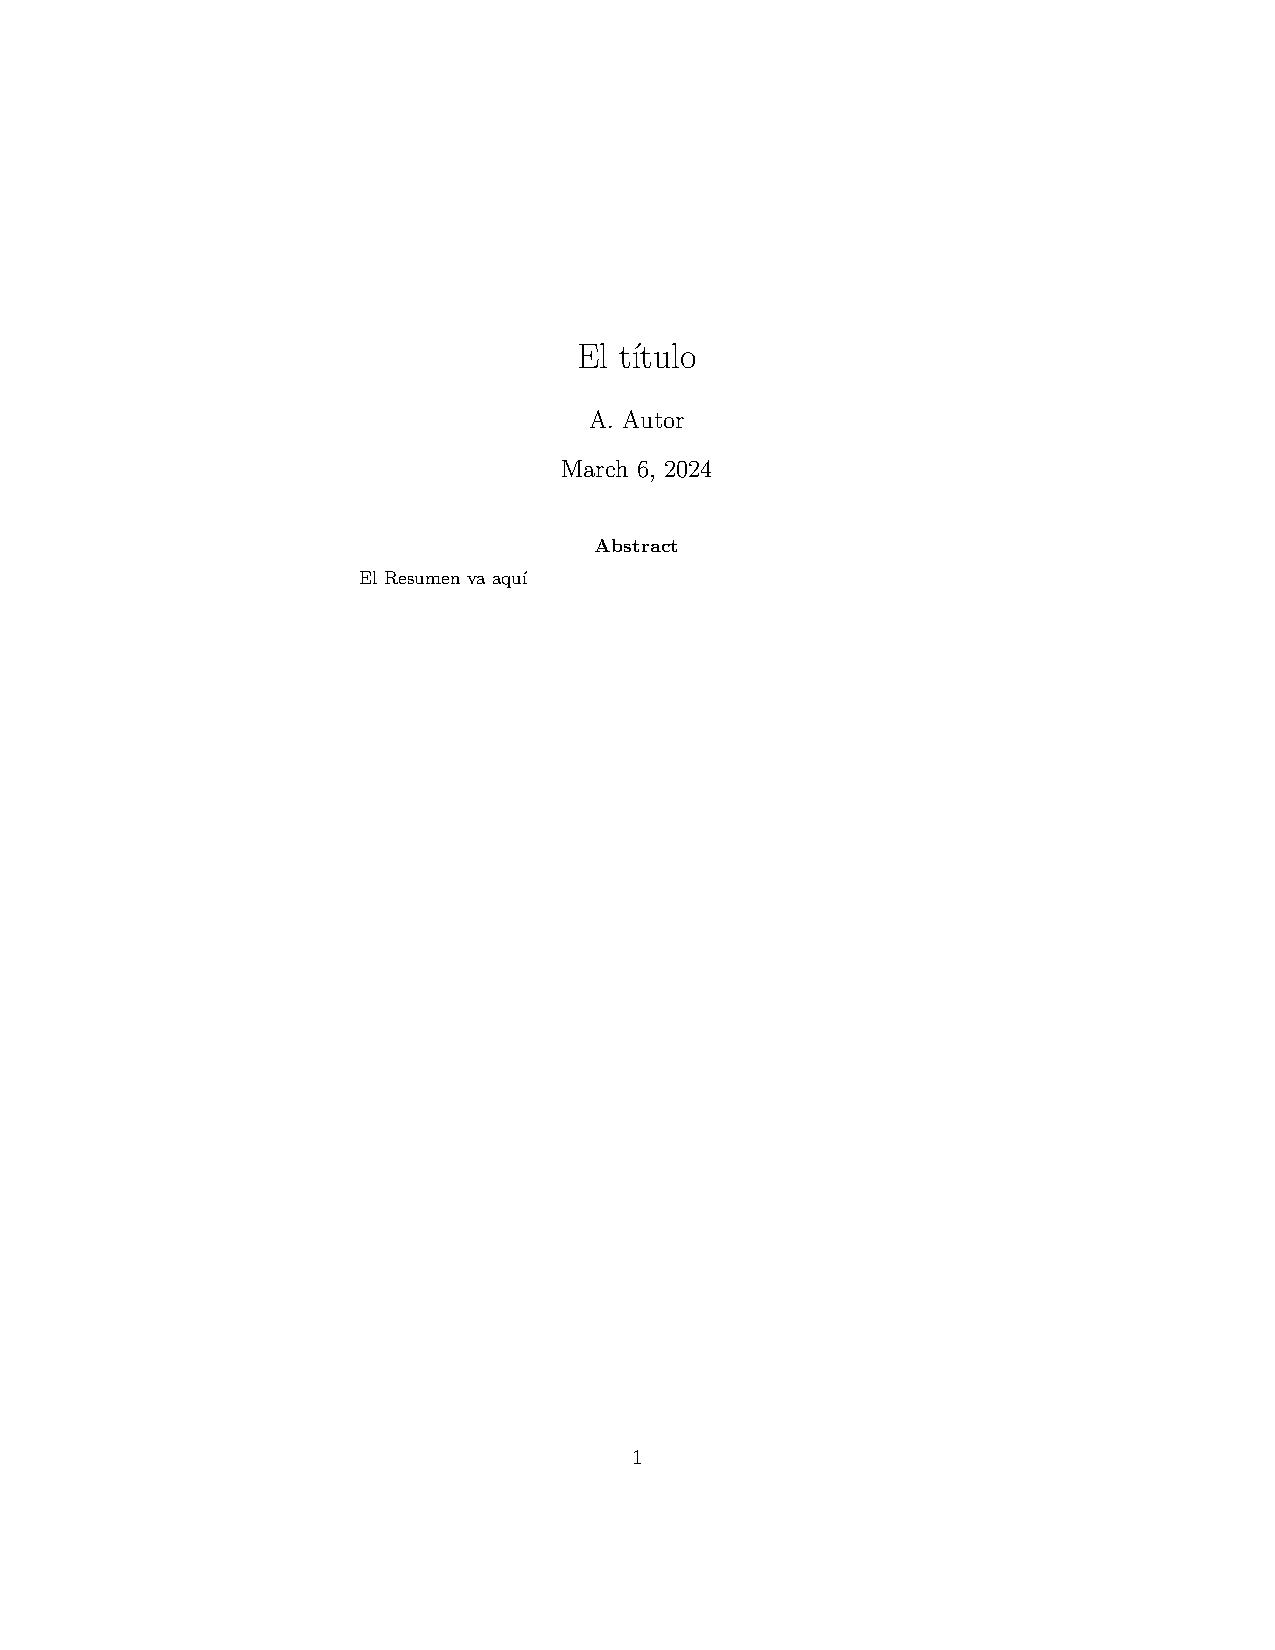
\includegraphics[width=\textwidth,clip,trim=2.2in 7in 2.2in 2in]{structure-title.pdf}
  \end{minipage}
\end{frame}

\begin{frame}{Secciones}
  \begin{itemize}{\small
    \item Solo utilice \cmdbs{section} y \cmdbs{subsection}.
    \item ¿Pueden adivinar qué hacen los comandos \cmdbs{section*} y \cmdbs{subsection*}?
    }\end{itemize}
  \begin{minipage}{0.55\linewidth}
    \inputminted[fontsize=\scriptsize,frame=single,resetmargins]{latex}%
    {structure-sections.tex}
  \end{minipage}
  \begin{minipage}{0.35\linewidth}
    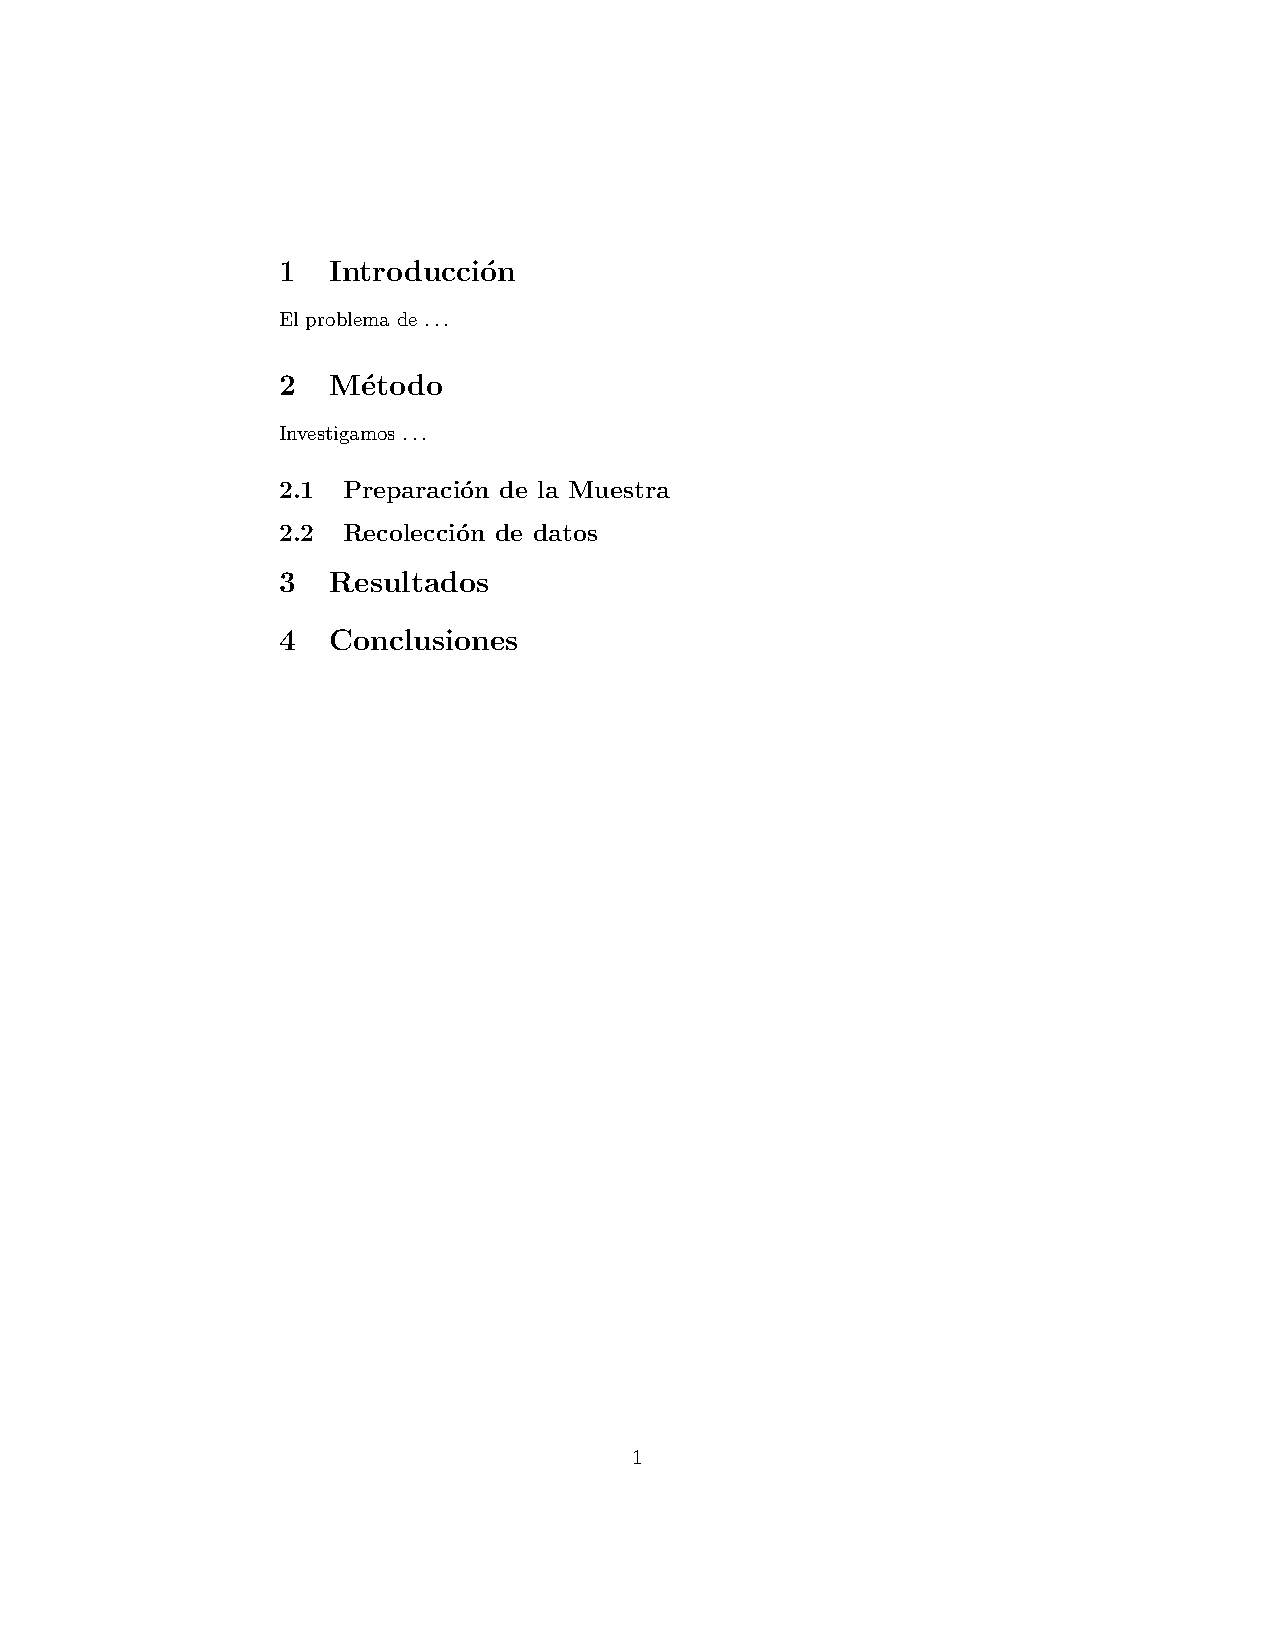
\includegraphics[width=\textwidth,clip,trim=1.5in 6in 4in 1in]{structure-sections.pdf}
  \end{minipage}
\end{frame}

\begin{frame}[fragile]{Etiquetas y Referencias Cruzadas}
  \begin{itemize}{\small
    \item Utilice \cmdbs{label} y \cmdbs{ref} para la numeración automática.
    \item El paquete \bftt{amsmath} proporciona \cmdbs{eqref} para
      las referencias de ecuaciones.
    }\end{itemize}
  \begin{minipage}{0.55\linewidth}
    \inputminted[fontsize=\scriptsize,frame=single,resetmargins]{latex}%
    {structure-crossref.tex}
  \end{minipage}
  \begin{minipage}{0.35\linewidth}
    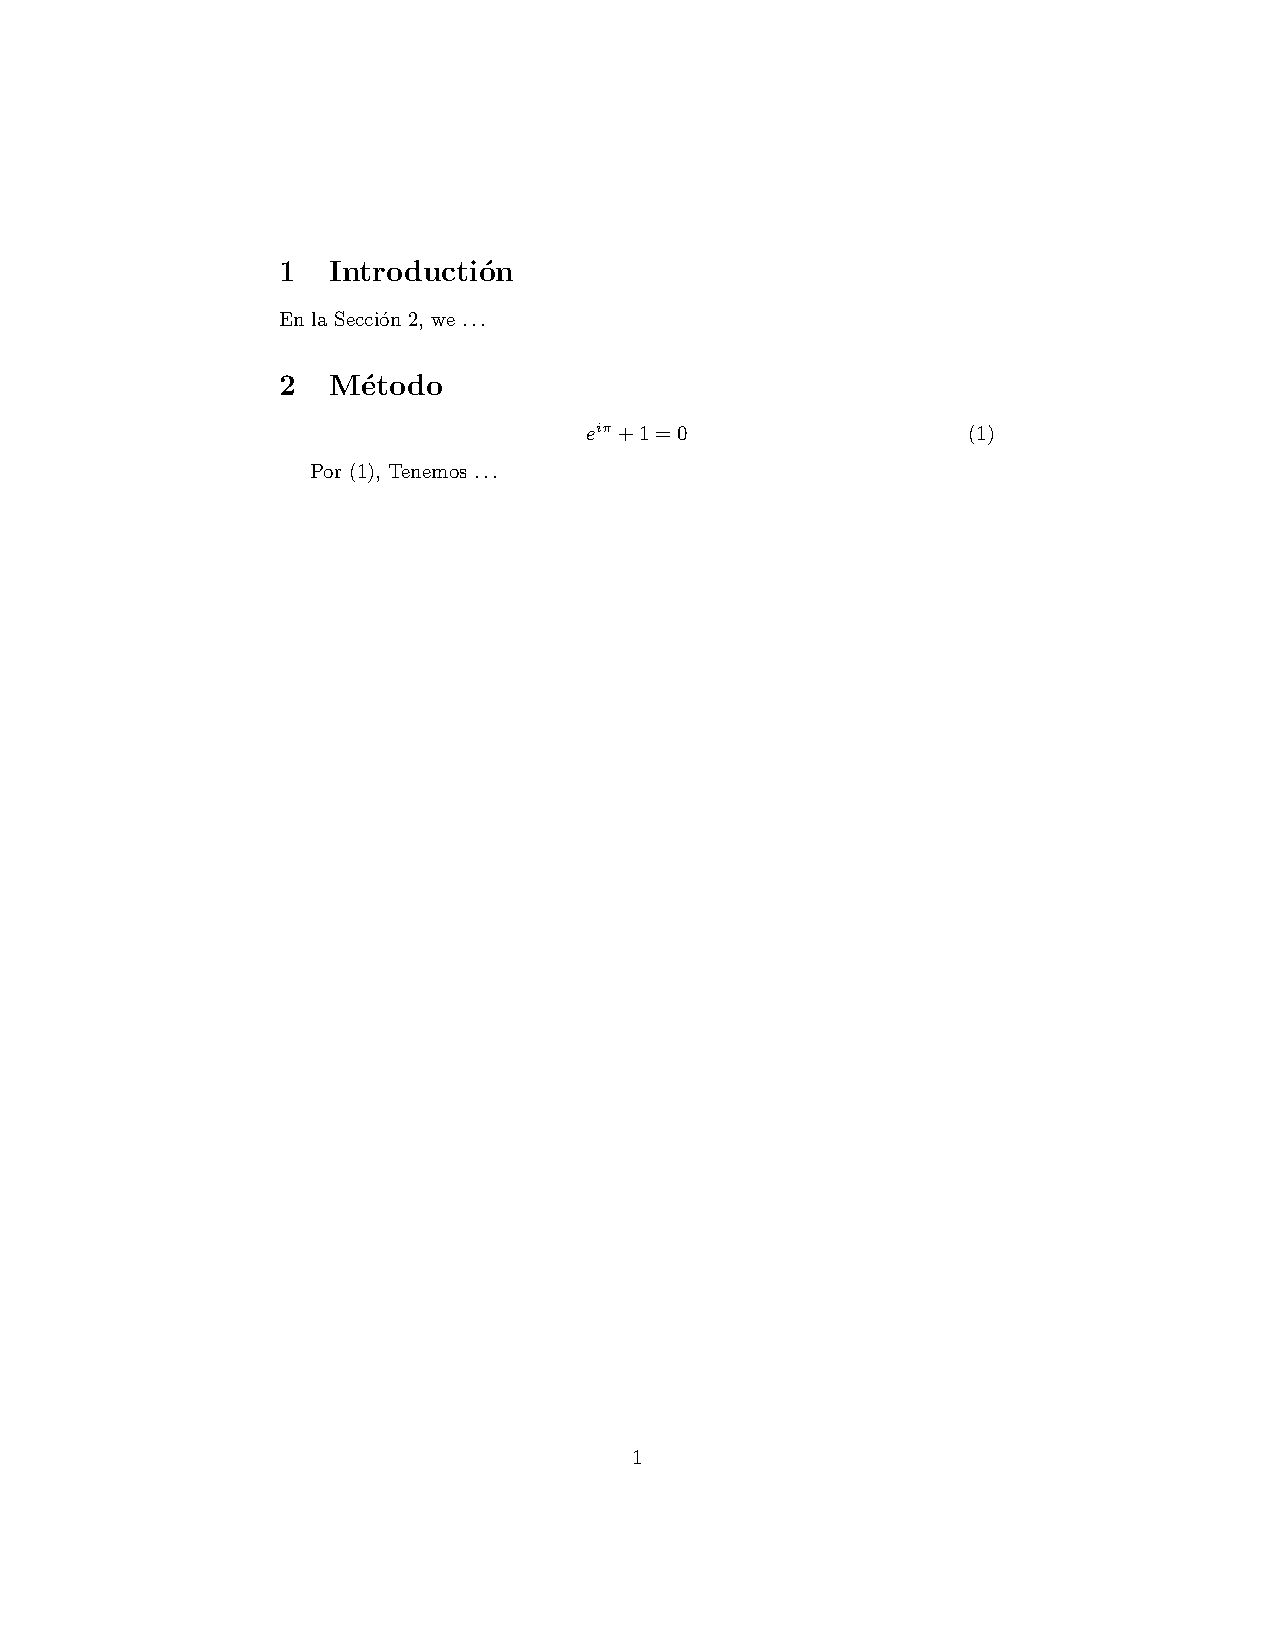
\includegraphics[width=\textwidth,clip,trim=1.8in 6in 1.6in 1in]{structure-crossref.pdf}
  \end{minipage}
\end{frame}

\begin{frame}[fragile]{Ejercicio de Documentos Estructurados}
  \begin{block}{Escriba este pequeño artículo en \LaTeX:
      \footnote{Desde \url{http://pdos.csail.mit.edu/scigen/}, un
        generador aleatorio de artículos.}}
    \begin{center}
      \fbox{\href{\fileuri/structure-exercise-solution.pdf}{%
          Click para abrir el artículo}}
    \end{center}
    Haga su versión del artículo mirando el documento original. Utilice
     \cmdbs{ref} y \cmdbs{eqref} para evitar escribir explícitamente
     la sección y el número de ecuación dentro del texto.
  \end{block}
 
\end{frame}

%---
\section{Figuras}
\begin{frame}[fragile]{Figuras}
  \begin{itemize}
  \item Requiere del paquete \bftt{graphicx}, que proporciona el
    comando \cmdbs{includegraphics}.
  \item Los formatos gráficos soportados incluyen JPEG, PNG y PDF.
  \end{itemize}
  \begin{exampletwouptiny}

\includegraphics[
width=0.5\textwidth]{logo_la}


\includegraphics[
width=0.3\textwidth,
angle=270]{logo_la}
  \end{exampletwouptiny}
  
  \tiny{Imagen desde \url{http://www.andy-roberts.net/writing/latex/importing_images}}
\end{frame}

\begin{frame}[fragile]{Figuras: Argumentos Opcionales}
  \begin{itemize}
  \item Utilizamos corchetes  \keystrokebftt{[} \keystrokebftt{]} para
    los argumentos opcionales, en lugar de las llaves \keystrokebftt{\{} \keystrokebftt{\}}.
  \item \cmdbs{includegraphics} acepta argumentos opcionales que
    permiten transformar la imagen cuando se incluya. Por ejemplo,
    \bftt{width=0.3\cmdbs{textwidth}}  hace que la imagen ocupe el
    30\% del ancho total asignado para el texto (\cmdbs{textwidth}).
  \item \cmdbs{documentclass} también acepta argumentos
    opcionales. Por ejemplo:
    \mint{latex}|\documentclass[12pt,twocolumn]{article}|
    \vskip 3ex
    hace al texto más grande (12pt) y lo coloca en dos columnas.
  \item ¿Dónde encontramos información sobre estas cosas? Vea las
    diapositivas hasta el final para obtener enlaces a más información.
  \end{itemize}
\end{frame}

\subsection[fragile]{}
\begin{frame}{Figuras Flotantes}
  \begin{itemize}
  \item Permita que \LaTeX{} decida dónde ubicar las figuras.
  \item Puede también darle a la figura un título, una etiqueta y así
    ser referenciado con \cmdbs{ref}.
  \end{itemize}
  \begin{minipage}{0.55\linewidth}
    \inputminted[fontsize=\scriptsize,frame=single,resetmargins]{latex}%
    {media-graphics.tex}
  \end{minipage}
  \begin{minipage}{0.35\linewidth}
    
\includegraphics[width=\textwidth,clip,trim=2in 5in 3in 1in]{media-graphics.pdf}
  \end{minipage}
\end{frame}

%---
\section{Tablas}
\begin{frame}[fragile]{Tablas}
  \begin{itemize}
  \item Las tablas en \LaTeX{} requieren un tiempo para acostumbrarse.
%  \item Utilice el entorno \bftt{tabular} desde el paquete
%\bftt{tabularx}.
  \item El argumento especifica la alineación de las columnas ---
\textbf{l}eft, \textbf{r}ight, \textbf{r}ight.
    \begin{exampletwouptiny}
\begin{tabular}{lrr}
  Art.   & Cant. & Uni. \$ \\
  DVD    & 1     & 19.99   \\
  Sonido & 2     & 39.99   \\
  Cable  & 3     & 1.99    \\
\end{tabular}
    \end{exampletwouptiny}
  \item También se especifican las líneas verticales; utilice el
comando \cmdbs{hline} para las líneas horizontales.
    \begin{exampletwouptiny}
\begin{tabular}{|l|r|r|}    \hline
  Art.   & Cant. & Uni.\$ \\\hline
  DVD    & 1     & 19.99  \\
  Sonido & 2     & 39.99  \\
  Cable  & 3     & 1.99   \\\hline
\end{tabular}
    \end{exampletwouptiny}
  \item Utilice un ampersand \keystrokebftt{\&} para separarlas
columnas y una doble barra invertida
\keystrokebftt{\bs}\keystrokebftt{\bs} para comenzar una nueva
fila(como en el entorno \bftt{align*} visto en la Parte 1).
  \end{itemize}
\end{frame}

%---
\section{Bibliografías}
\begin{frame}[fragile]{bib\TeX}
  \begin{itemize}
  \item Colocar las referencias en un archivo \bftt{.bib} en el
    formato de base de datos  `bibtex':
    \inputminted[fontsize=\scriptsize,frame=single]{latex}{bib-example.bib}
  \item La mayoría de los gestores de referencias pueden exportar al
    formato bibtex.
  \end{itemize}
\end{frame}

\begin{frame}[fragile]{bib\TeX}
  \begin{itemize}
  \item Cada entrada en el archivo  \bftt{.bib} tiene una \emph{clave}
    que puede usar para ser citado en el documento. Por ejemplo,
    \bftt{Jacobson1999Towards} es la clave para este artículo:
    \begin{minted}[fontsize=\small,frame=single]{latex}
@Article{Jacobson1999Towards,
  author = {Van Jacobson},
  ...
}
    \end{minted}
  \item Es recomendable utilizar una clave basada en el nombre, año y
    título del artículo.
  \item \LaTeX{} puede formatear automáticamente sus citas en el texto
    y generar una lista de referencias; basados en estilos estándares,
    y hasta se pueden diseñar sus propios estilos.
  \end{itemize}
\end{frame}

\begin{frame}[fragile]{bib\TeX}
  \begin{itemize}
  \item Utilice el paquete \bftt{natbib} \footnote{Hay un nuevo
      paquete con más características llamado \bftt{biblatex} pero la
      mayoría de las plantillas para artículos todavía utiliza
      \bftt{natbib}.} con \cmdbs{citet} y \cmdbs{citep}.
  \item Las referencias bibliográficas van al final del texto con el
    comando \cmdbs{bibliography}, y luego se especifica el estilo con
    \cmdbs{bibliographystyle}.
  \end{itemize}
  \begin{minipage}{0.55\linewidth}
    \inputminted[fontsize=\scriptsize,frame=single,resetmargins]{latex}%
    {bib-example.tex}
  \end{minipage}
  \begin{minipage}{0.35\linewidth}
    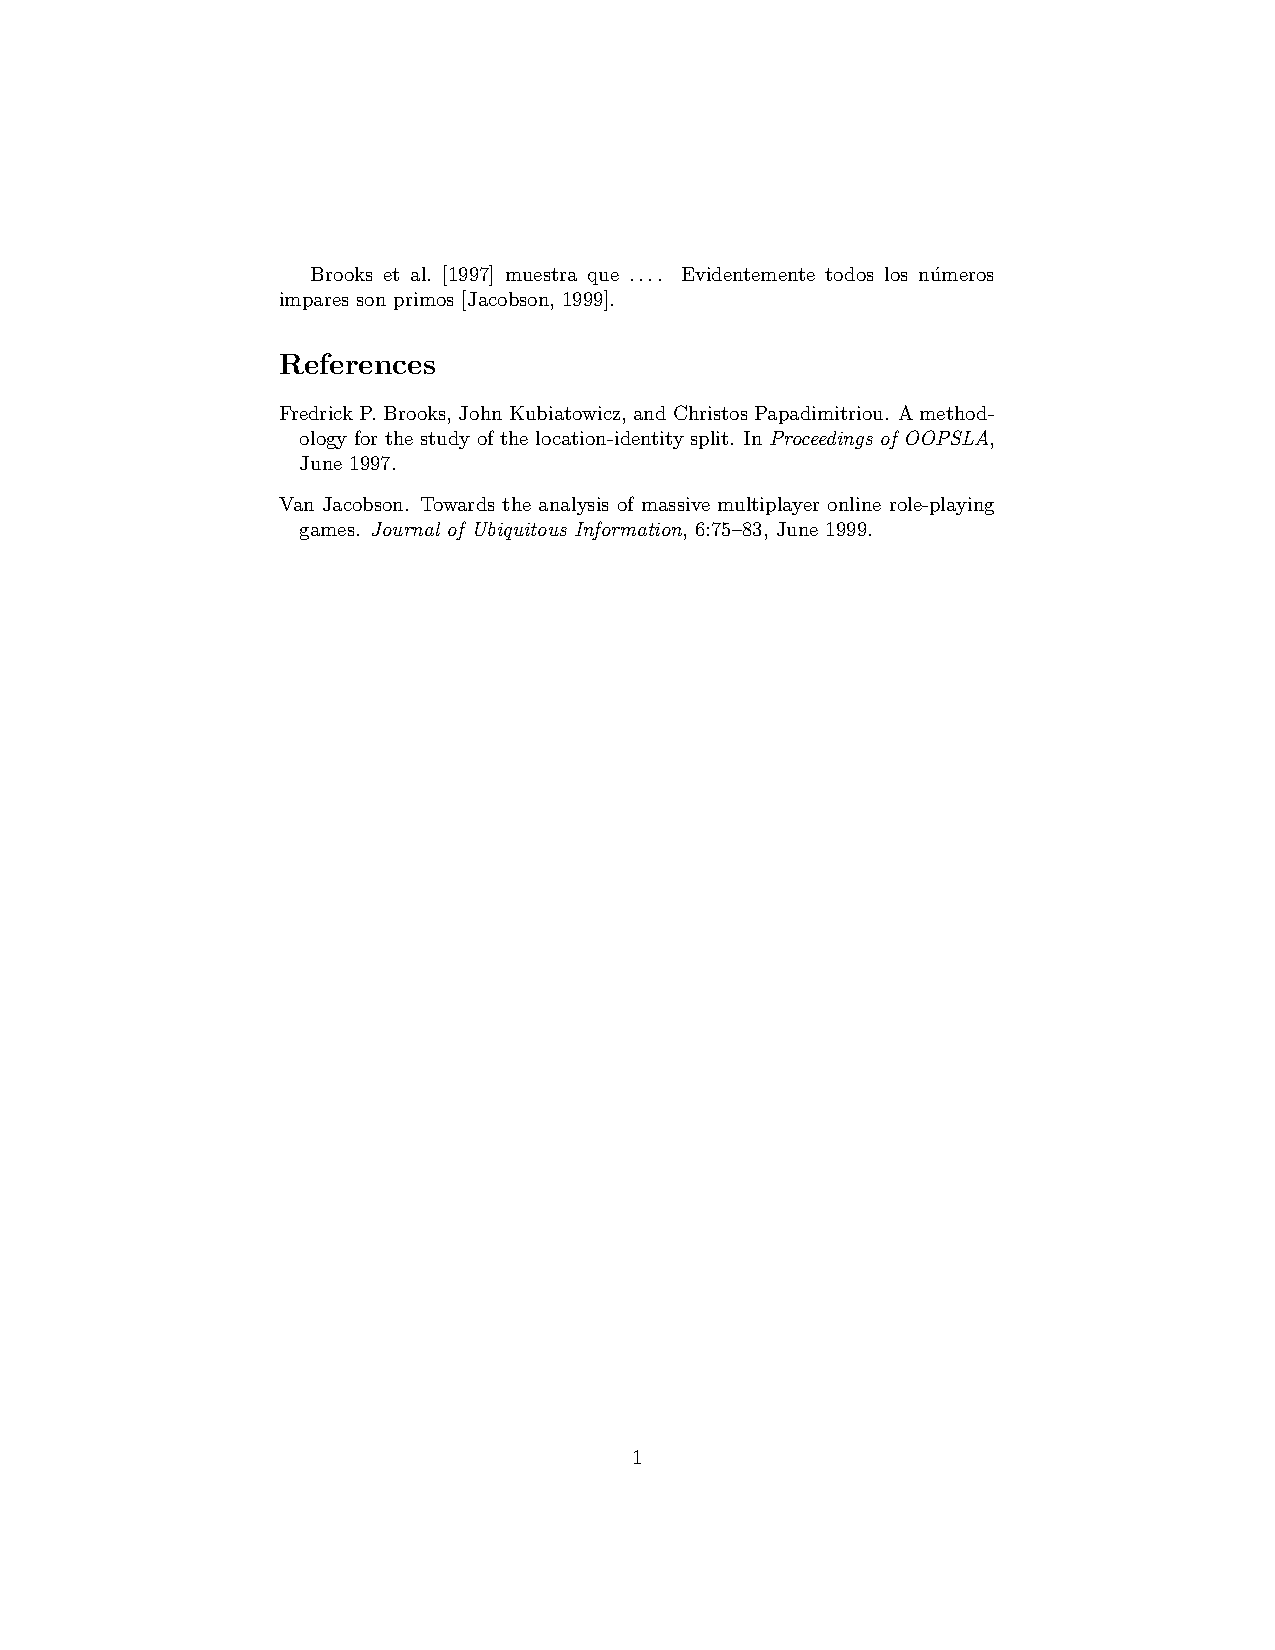
\includegraphics[width=\textwidth,clip,trim=1.8in 5in 1.8in 1in]{bib-example.pdf}
  \end{minipage}
\end{frame}


%
\end{document}


